\documentclass[a0,portrait,final]{a0poster}

\usepackage{calc}
\usepackage{epsfig}
\usepackage{xspace}
\usepackage{amsmath}
\usepackage{wrapfig}
\usepackage{multirow}
\usepackage{rotating}
\usepackage{arydshln}
\usepackage{booktabs}
\usepackage{multicol}
\usepackage{enumitem}
\usepackage{inconsolata}
\usepackage[english]{babel}
\usepackage{pstricks,pst-grad}
\usepackage{hyperref}
\usepackage{listings}
\usepackage{color}


\newrgbcolor{bluisti}{0.02 0.23 0.38}% #073B62 R7 G59 B98
\newrgbcolor{arancioneisti}{0.98 0.44 0.08}% #FC7216 R252 G114 B22
%\newrgbcolor{orangered}{1 0.14 0.00}%orangered rgb(100%, 14%, 0%
%\newrgbcolor{rosso}{0.80 0.00 0.00}%
%\newrgbcolor{yahoo}{0.40 0.00 0.60}%concord grape rgb(40%, 0%, 60%)
%\newrgbcolor{verde}{0.0 0.702 0.0}

\setlength{\columnsep}{1in}
\setlength{\parindent}{0.0cm}

\newcommand{\pbox}[3]{
	\begin{center}
	\psshadowbox[linewidth=2mm,framearc=0.1,framesep=1em,shadowsize=4mm,shadowcolor=lightgray,linecolor=#2]{
		\begin{minipage}[t][][t]{#1}{
			#3 %text
		}\end{minipage}
	}
	\end{center}
}

\newcommand{\dexter}[1]{{\sf Dexter}\xspace}

\newlength\ptitlespace
\setlength\ptitlespace{2.6cm}

\newcommand{\ptitle}[1]{
	\vspace{\ptitlespace}
	\pbox{0.92\columnwidth}{arancioneisti}{
		\begin{center}
		\textsc{\LARGE\bluisti{#1}} %text
		\end{center}
	}
	\vspace{0.5\ptitlespace}
}

\newcommand{\btitle}[1]{\begin{center} \Large{\textsc{#1}} \end{center} \vspace{1.5cm}}
	
\begin{document}
	\newlength\logosize
	\setlength\logosize{8cm}
	\pbox{0.96\textwidth}{arancioneisti}{
	\centering
	\begin{tabular}{ccc}
		\begin{minipage}[c]{\logosize}
		\centering
			
\includegraphics[width=5cm]{img/ucl.eps}
		\end{minipage}
	&
		\begin{minipage}[c]{0.98\textwidth-2\logosize}
		\centering\textsc{}
		\Huge \textsc{Bringing the Head Closer to the Tail\\ with Entity Linking}\\[8mm]
	\Large{Manisha Verma$^{1}$, Diego Ceccarelli$^{2,3}$}\\
	\Large{$^1$ UCL Department Of Computer Science}
	\Large{$^2$ ISTI-CNR, Pisa, Italy}\hspace{2cm}\Large{$^3$ IMT Lucca}\\
	
		\end{minipage}
	& 

	\begin{minipage}[c]{\logosize}
	\centering
	
	\end{minipage}
		\begin{minipage}[c]{\logosize}
		\centering
		
\includegraphics[width=9cm]{img/logohpc.eps}
		\includegraphics[width=5cm]{img/logoisti.eps}
		\end{minipage}
	\end{tabular}
	}


\vfill
\large


\begin{multicols}{2}

\ptitle{Entity Linking Problem}

The entity linking task aims at identifying, given a plain document, the small fragments of text (interchangeably called \emph{mentions} or \emph{spots}) referring to any \emph{named entity} that is listed in a given knowledge base, e.g. Wikipedia. The ambiguity of natural language makes it a non trivial task. The same entity can be in fact mentioned with different text fragments, e.g., ``President Kennedy'' or ``John F. Kennedy''. On the other hand, the same mention may refer to different entities, e.g., ``Michael Collins'' may refer to either the well known astronaut, or to the Irish leader and president of the Irish provisional government in 1922.

\vspace{5mm}
\begin{center}
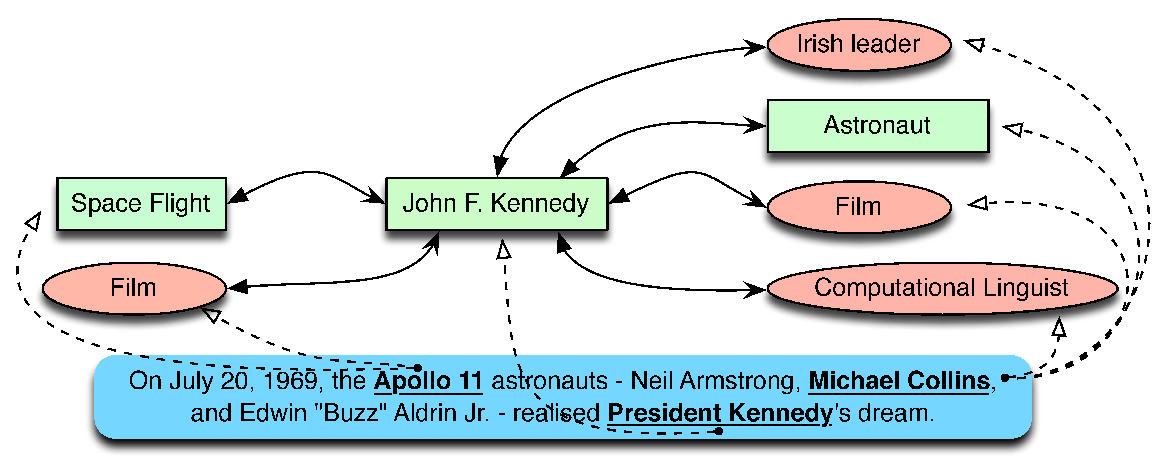
\includegraphics[width=0.92\columnwidth]{img/annotation-example.eps}
\end{center}

The annotation is usually organized in three subtasks:
\begin{enumerate}
	\item \textbf{Spotting}: discover the fragments that could refer to an entity. A set of candidate mentions is detected, and for each mention a list of candidate entities is produces;
	\item \textbf{Disambiguation}: for each spot associated with more than one candidate, a single entity is selected to be linked to the spot;
	\item \textbf{Ranking}: the list of entites detected is ranked according to some policy, e.g. annotation confidence. 
\end{enumerate}


% \ptitle{Motivations}
% Several entity linking algorithms were recently proposed for annotating documents with entities. Performing a fair comparison among these techniques is very hard. To the best of our knowledge, only a few authors released the source code of their algorithms or provide
% a REST API for annotating documents using their method. As a result, evaluating today the performance of a method on a single subtask, comparing different techniques or mixing different strategies together is difficult.
%
% \vspace{4mm}
% \textbf{We strongly believe that it is important to share a unique framework where each subtask is well separated and easy to isolate in order to study its performance, perform fair comparisons and improve the state of the art.}
%
%
% \ptitle{Dexter Framework}
%
% In this work we present a new open source framework, called Dexter, that implements some popular algorithms and provides several tools useful to develop an entity linking technique.
%
% % \vspace{10mm}
% % \begin{center}
% % \includegraphics[width=0.20\columnwidth]{img/dexter-logo.eps}
% % \end{center}
%
% \vspace{10mm}
% \begin{center}
% \includegraphics[width=0.80\columnwidth]{img/screenshot.eps}
% \end{center}
%
% \ptitle{Dexter Architecture}
%
% Dexter is developed in Java and is organized in several Maven modules.
%
% \vspace{10mm}
% \begin{center}
% \includegraphics[width=0.8\columnwidth]{./img/dexter-architecture.eps}
% \end{center}
%
% \ptitle{Plug and Play}
%
% \lstset{language=Java,
%  		   basicstyle=\fontsize{24}{26}\ttfamily,
%            keywordstyle=\color{blue}\ttfamily,
%            stringstyle=\color{red}\ttfamily,
%            commentstyle=\color{green}\ttfamily}
% \begin{lstlisting}
% public class TopScoreEntityDisambiguator implements Disambiguator {
%         @Override
%         public EntityMatchList disambiguate(SpotMatchList sml) {
%                 EntityMatchList eml = new EntityMatchList();
%                 for (SpotMatch match : sml){
%                         EntityMatchList list = match.getEntities();
%                         if (! list.isEmpty()){
%                                 list.sort();
%                                 eml.add(list.get(0));
%                         }
%                 }
%                 return eml;
%         }
% }
% \end{lstlisting}
%
% \ptitle{Conclusion and Future Work}
%
% \begin{itemize}
% \item We implemented two state-of-the-art methods in Dexter: TAGME and Wikiminer. We plan to implement several other state of the art approaches in order to show their performance and efficiency on a wide range of datasets;
% \item We plan to investigate the performance of the entity linking methods on different evaluation datasets. We have recently released
% \textbf{Elianto}  a web-deployed tool that allows to crowdsource the creation of manually annotated datasets;
% \item We plan to support different Wikipedia languages (actually only English is supported);
% \item We intend to improve the performance of the annotator, in terms of result's quality, response time and resource usage.
% \end{itemize}
%
% \ptitle{Fork me on Github!}
%
% The code is available on Github at the following address:
% \begin{itemize}
% 	\item \url{https://github.com/diegoceccarelli/dexter}
% \end{itemize}
%
% A demo webapp and some other useful informations can be found here:
% \begin{itemize}
% 	\item \url{http://www.dxtr.it}
% \end{itemize}

\end{multicols}
\vfill
\centering
\begin{minipage}[c]{\textwidth}
\rule{\textwidth}{1pt}
\textit{ESAIR '14  -- 7$^\textit{th}$ International Workshop on Exploiting Semantic Annotations in Information Retrieval. November 7, 2014. Shanghai, China.}
%\textit{ESAIR '14  -- The 23\emph{rd} ACM Conference on Information \& Knowledge Management. November 3-7, 2014. Shanghai, China}
\end{minipage}

\end{document}